\documentclass[a4paper,11pt]{book}
%\documentclass[a4paper,twoside,11pt,titlepage]{book}
\usepackage{lmodern}
\usepackage{listings}
\usepackage[utf8]{inputenc}
\usepackage[spanish]{babel}
\usepackage{xspace}
\usepackage{amsthm}
\usepackage{amssymb}
\usepackage{url}          % para que \url{} funcione bien en los campos howpublished
\usepackage[numbers]{natbib}
\usepackage[hidelinks]{hyperref}
\usepackage{listings}
% \usepackage[style=list, number=none]{glossary} %
%\usepackage{titlesec}
%\usepackage{pailatino}
\usepackage{float}
\usepackage{amsmath}
\usepackage{amsfonts}
\usepackage{xcolor}
\usepackage{booktabs}
\usepackage{algorithm}
\usepackage{algorithmic}
\usepackage{amsthm}
\usepackage{graphicx}

% Configuración de decimales y tablas
\decimalpoint
\usepackage{dcolumn}
\newcolumntype{.}{D{.}{\esperiod}{-1}}
\makeatletter
\addto\shorthandsspanish{\let\esperiod\es@period@code}
\makeatother


% Encabezados y pie de página
%\usepackage[chapter]{algorithm}
\RequirePackage{verbatim}
%\RequirePackage[Glenn]{fncychap}
\usepackage{fancyhdr}
\usepackage{graphicx}
\usepackage{afterpage}
\usepackage{colortbl}
\usepackage{longtable}
\usepackage[stable]{footmisc}
\usepackage{pdfpages}
%referencia

% ********************************************************************
% Re-usable information
% ********************************************************************
\newcommand{\myTitle}{Fundamentos teóricos de las curvas elípticas y su aplicación en criptografía\xspace}
\newcommand{\myDegree}{Grado en Ingeniería Informática\xspace}
\newcommand{\myName}{Leon Elliott Fuller\xspace}
\newcommand{\myProf}{Jesús García Miranda\xspace}
\newcommand{\myOtherProf}{Nombre Apllido1 Apellido2 (tutor2)\xspace}
%\newcommand{\mySupervisor}{Put name here\xspace}
\newcommand{\myFaculty}{Escuela Técnica Superior de Ingenierías Informática y de
Telecomunicación\xspace}
\newcommand{\myFacultyShort}{E.T.S. de Ingenierías Informática y de
Telecomunicación\xspace}
\newcommand{\myDepartment}{Departamento de Computación y Sistemas Inteligentes\xspace}
\newcommand{\myUni}{\protect{Universidad de Granada}\xspace}
\newcommand{\myLocation}{Granada\xspace}
\newcommand{\myTime}{\today\xspace}
\newcommand{\myVersion}{Version 0.1\xspace}
\newcommand{\myNIE}{...\xspace}

\hypersetup{
    pdfauthor = {\myName (leonfuller@correo.ugr.es)},
    pdftitle = {\myTitle},
    pdfsubject = {},
    pdfkeywords = {palabra_clave1, palabra_clave2, palabra_clave3, ...},
    pdfcreator = {LaTeX con el paquete ....},
    pdfproducer = {pdflatex},
}

%\hyphenation{}


%\usepackage{doxygen/doxygen}
%\usepackage{pdfpages}
\usepackage{url}
\usepackage{colortbl,longtable}
\usepackage[stable]{footmisc}
%\usepackage{index}

%\makeindex
%\usepackage[style=long, cols=2,border=plain,toc=true,number=none]{glossary}
% \makeglossary

% Definición de comandos que me son tiles:
%\renewcommand{\indexname}{Índice alfabético}
%\renewcommand{\glossaryname}{Glosario}

\pagestyle{fancy}
\fancyhf{}
\fancyhead[LO]{\leftmark}
\fancyhead[RE]{\rightmark}
\fancyhead[RO,LE]{\textbf{\thepage}}
\renewcommand{\chaptermark}[1]{\markboth{\textbf{#1}}{}}
\renewcommand{\sectionmark}[1]{\markright{\textbf{\thesection. #1}}}

\setlength{\headheight}{1.5\headheight}

\newcommand{\HRule}{\rule{\linewidth}{0.5mm}}
%Definimos los tipos teorema, ejemplo y definición podremos usar estos tipos
%simplemente poniendo \begin{teorema} \end{teorema} ...
\newtheorem{teorema}{Teorema}[chapter]
\newtheorem{ejemplo}{Ejemplo}[chapter]
\newtheorem{definicion}{Definición}[chapter]
\newtheorem{remark}{Observación}[chapter]
\newtheorem{corollary}{Corolario}[chapter]

\definecolor{gray97}{gray}{.97}
\definecolor{gray75}{gray}{.75}
\definecolor{gray45}{gray}{.45}
\definecolor{gray30}{gray}{.94}

\lstset{ frame=Ltb,
     framerule=0.5pt,
     aboveskip=0.5cm,
     framextopmargin=3pt,
     framexbottommargin=3pt,
     framexleftmargin=0.1cm,
     framesep=0pt,
     rulesep=.4pt,
     backgroundcolor=\color{gray97},
     rulesepcolor=\color{black},
     %
     stringstyle=\ttfamily,
     showstringspaces = false,
     basicstyle=\scriptsize\ttfamily,
     commentstyle=\color{gray45},
     keywordstyle=\bfseries,
     %
     numbers=left,
     numbersep=6pt,
     numberstyle=\tiny,
     numberfirstline = false,
     breaklines=true,
   }
 
% minimizar fragmentado de listados
\lstnewenvironment{listing}[1][]
   {\lstset{#1}\pagebreak[0]}{\pagebreak[0]}

\lstdefinestyle{CodigoC}
   {
	basicstyle=\scriptsize,
	frame=single,
	language=C,
	numbers=left
   }
\lstdefinestyle{CodigoC++}
   {
	basicstyle=\small,
	frame=single,
	backgroundcolor=\color{gray30},
	language=C++,
	numbers=left
   }

 
\lstdefinestyle{Consola}
   {basicstyle=\scriptsize\bf\ttfamily,
    backgroundcolor=\color{gray30},
    frame=single,
    numbers=none
   }


\newcommand{\bigrule}{\titlerule[0.5mm]}


%Para conseguir que en las páginas en blanco no ponga cabecerass
\makeatletter
\def\clearpage{%
  \ifvmode
    \ifnum \@dbltopnum =\m@ne
      \ifdim \pagetotal <\topskip
        \hbox{}
      \fi
    \fi
  \fi
  \newpage
  \thispagestyle{empty}
  \write\m@ne{}
  \vbox{}
  \penalty -\@Mi
}
\makeatother

\usepackage{pdfpages}
\bibliographystyle{unsrtnat}
\begin{document}
\begin{titlepage}
 
 
    \newlength{\centeroffset}
    \setlength{\centeroffset}{-0.5\oddsidemargin}
    \addtolength{\centeroffset}{0.5\evensidemargin}
    \thispagestyle{empty}
    
    \noindent\hspace*{\centeroffset}\begin{minipage}{\textwidth}
    
    \centering
    
\includegraphics[width=0.9\textwidth]{imagenes/logo_ugr.jpg}\\[1.4cm]
    
    \textsc{ \Large TRABAJO FIN DE GRADO\\[0.2cm]}
    \textsc{ INGENIERÍA INFORMÁTICA}\\[1cm]
    % Upper part of the page
    % 
    % Title
    {\Huge\bfseries {\myTitle}\\
    }
    \noindent\rule[-1ex]{\textwidth}{3pt}\\[3.5ex]
    {\large\bfseries Un estudio un detalle sobre Curvas Ellípticas aplicadas a la Criptografía}
    \end{minipage}
    
    \vspace{2.5cm}
    \noindent\hspace*{\centeroffset}\begin{minipage}{\textwidth}
    \centering
    
    \textbf{Autor}\\ {Leon Elliott Fuller}\\[2.5ex]
    \textbf{Directores}\\
    {Jesús García Miranda\\[2cm]}
    
\includegraphics[width=0.3\textwidth]{imagenes/etsiit_logo.png}\\[0.1cm]
    \textsc{Escuela Técnica Superior de Ingenierías Informática y de Telecomunicación}\\
    \textsc{---}\\
    Granada, Abril de 2025
    \end{minipage}
    %\addtolength{\textwidth}{\centeroffset}
    %\vspace{\stretch{2}}
    \end{titlepage}
    
    
    
\chapter*{}
%\thispagestyle{empty}
%\cleardoublepage

%\thispagestyle{empty}

\begin{titlepage}
 
 
    \setlength{\centeroffset}{-0.5\oddsidemargin}
    \addtolength{\centeroffset}{0.5\evensidemargin}
    \thispagestyle{empty}
    
    \noindent\hspace*{\centeroffset}\begin{minipage}{\textwidth}
    
    \centering
    %
\includegraphics[width=0.9\textwidth]{imagenes/logo_ugr.jpg}\\[1.4cm]
    
    %\textsc{ \Large PROYECTO FIN DE CARRERA\\[0.2cm]}
    %\textsc{ INGENIERÍA EN INFORMÁTICA}\\[1cm]
    % Upper part of the page
    % 
    
     \vspace{3.3cm}
    
    %si el proyecto tiene logo poner aquí
    
\includegraphics{imagenes/logo.png} 
     \vspace{0.5cm}
    
    % Title
    
    {\Huge\bfseries \myTitle\\}
    \noindent\rule[-1ex]{\textwidth}{3pt}\\[3.5ex]
    {\large\bfseries Un estudio un detalle sobre Curvas Ellípticas aplicadas a la Criptografía.\\[4cm]}
    \end{minipage}
    
    \vspace{2.5cm}
    \noindent\hspace*{\centeroffset}\begin{minipage}{\textwidth}
    \centering
    
    \textbf{Autor}\\ {Leon Elliott Fuller}\\[2.5ex]
    \textbf{Directores}\\
    Jesús García Miranda\\[2cm]
    %
\includegraphics[width=0.15\textwidth]{imagenes/tstc.png}\\[0.1cm]
    %\textsc{Departamento de Teoría de la Señal, Telemática y Comunicaciones}\\
    %\textsc{---}\\
    %Granada, mes de 201
    \end{minipage}
    %\addtolength{\textwidth}{\centeroffset}
    \vspace{\stretch{2}}
    
     
    \end{titlepage}
    
    
    



\cleardoublepage
\thispagestyle{empty}

\begin{center}
{\large\bfseries Elliptic Curve Criptography: Un estudio un detalle sobre Curvas Ellípticas aplicadas a la Criptografía}\\
\end{center}
\begin{center}
Leon Elliott Fuller\\
\end{center}

%\vspace{0.7cm}
\noindent{\textbf{Palabras clave}: palabra\_clave1, palabra\_clave2, palabra\_clave3, ......}\\

\vspace{0.7cm}
\noindent{\textbf{Resumen}}\\

Poner aquí el resumen.
\cleardoublepage


\thispagestyle{empty}


\begin{center}
{\large\bfseries Project Title: Project Subtitle}\\
\end{center}
\begin{center}
First name, Family name (student)\\
\end{center}

%\vspace{0.7cm}
\noindent{\textbf{Keywords}: Keyword1, Keyword2, Keyword3, ....}\\

\vspace{0.7cm}
\noindent{\textbf{Abstract}}\\

Write here the abstract in English.

\chapter*{}
\thispagestyle{empty}

\noindent\rule[-1ex]{\textwidth}{2pt}\\[4.5ex]

Yo, \textbf{Leon Elliott Fuller}, alumno de la titulación Ingeniería Informática de la \textbf{Escuela Técnica Superior
de Ingenierías Informática y de Telecomunicación de la Universidad de Granada}, con NIE Y3299550F, autorizo la
ubicación de la siguiente copia de mi Trabajo Fin de Grado en la biblioteca del centro para que pueda ser
consultada por las personas que lo deseen. Todo el código
fuente así como este documento en formato LaTeX se puede encontrar en
el siguiente repositorios de GitHub

\vspace{6cm}

\noindent Fdo: Leon Elliott Fuller

\vspace{2cm}

\begin{flushright}
Granada a X de mayo de 2025.
\end{flushright}


\chapter*{}
\thispagestyle{empty}

\noindent\rule[-1ex]{\textwidth}{2pt}\\[4.5ex]

D. \textbf{Jesús García Miranda}, Profesor del Área de XXXX del Departamento YYYY de la Universidad de Granada.

\vspace{0.5cm}

\vspace{0.5cm}

\textbf{Informa:}

\vspace{0.5cm}

Que el presente trabajo, titulado \textit{\textbf{Título del proyecto, Subtítulo del proyecto}},
ha sido realizado bajo su supervisión por \textbf{Leon Elliott Fuller}, y autorizamos la defensa de dicho trabajo ante el tribunal
que corresponda.

\vspace{0.5cm}

Y para que conste, expiden y firman el presente informe en Granada a X de mayo de 2025.

\vspace{1cm}

\textbf{El tutor:}

\vspace{5cm}

\noindent \textbf{Jesús García Miranda}

\chapter*{Agradecimientos}
\thispagestyle{empty}

       \vspace{1cm}


Poner aquí agradecimientos...


\frontmatter
\tableofcontents
\listoffigures
\listoftables
\mainmatter
%\setlength{\parskip}{5pt}

\part{Introducción}
\chapter{Introducción}

\section{Contexto histórico y motivación}
La comunicación confidencial entre sujetos ha sido una necesidad constante a lo largo de la historia. Cuando los mensajes debían transmitirse de forma no presencial o transportarse físicamente, surgía el reto de asegurar que ninguna entidad externa pudiera leerlos o alterarlos sin ser detectada.

Ya en la Antigüedad, civilizaciones como la espartana emplearon la “Escítala” en el siglo V a. C., un dispositivo de transposición que cifraba mensajes al enrollarlos en un cilindro. Más tarde, los griegos documentaron con Polibio un sistema de sustitución basado en el orden de las letras, y Roma adoptó el famoso Cifrado César, que desplazaba el alfabeto para ocultar información militar y diplomática.

Durante el Renacimiento, el cifrado avanzó hacia métodos más sofisticados, como el de Leon Battista Alberti que introdujo en 1465 la idea del cifrado polialfabético mediante discos concéntricos, lo que supuso un gran avance en esa época. Blaise de Vigenère perfeccionó esta técnica en el siglo XVI con una tabla que combinaba alfabetos de forma periódica, y en Europa se publicaron tratados (como el \emph{Cryptomenytices et Cryptographiae} de Selenus) que difundieron estos métodos entre cortes y ejércitos.

El siglo XX presenció el mayor salto tecnológico, donde se partió de los cifrados manuales de la Primera Guerra Mundial hasta la aparición de máquinas electromecánicas como la Enigma alemana en la Segunda Guerra Mundial, una máquina de rotores que automatizaba los cálculos que era necesario realizar para las operaciones de cifrado y descifrado de mensajes. El descifrado de Enigma por los criptógrafos aliados no solo cambió el curso del conflicto, sino que marcó el inicio de la era del cálculo automatizado al servicio de la criptografía. Tras la guerra, Claude Shannon sentó las bases teóricas de la información y la seguridad, y en los años 70 el NIST publicó el Estándar de Cifrado de Datos (DES), consolidando el cifrado simétrico en la informática moderna.

Sin embargo, todos los criptosistemas anteriores tenían un inconveniente, y es que todos se basaban en el hecho de que tanto la parte que descifraba como la que codificaba debían conocer el método de cifrado y la clave para descifrarlo. ¿Pero cómo se transmite la clave de forma segura? Por supuesto, con cifrado. Pero entonces, ¿cómo se puede enviar el cifrado, para que la entidad que descifra el mensaje pueda conocer dicho cifrado? Como se puede apreciar, dicho problema de la criptografía es un bucle infinito entre el cifrado y la distribución de claves que no se puede resolver con seguridad garantizada para todos los lectores deseados.

Hoy día, RSA y sistemas análogos sustentan protocolos críticos—HTTPS, correo firmado, servicios bancarios y más—pero presentan dos limitaciones crecientes:  
\begin{itemize}  
  \item \textbf{Tamaño de clave versus seguridad.} Para alcanzar un nivel de protección comparable al de cifrados simétricos de 128 bits, RSA requiere claves de varios miles de bits, lo que penaliza el rendimiento en cómputo y ancho de banda.  
  \item \textbf{Vulnerabilidad cuántica.} 
  Los algoritmos cuánticos plantean un desafío fundamental para la criptografía moderna. En particular, **Shor** demostró en 1994 que un ordenador cuántico suficientemente grande podría factorizar enteros y resolver problemas de logaritmo discreto en tiempo polinómico, lo que rompería sistemas como RSA, Diffie–Hellman e incluso ECC \cite{turn2search1}\cite{turn2search2}. Esta perspectiva ha impulsado la búsqueda de algoritmos resistentes a estos ataques cuánticos, así como la adopción de curvas elípticas de mayor seguridad y longitudes de clave incrementadas.  
\end{itemize}  

Estas limitaciones han impulsado la adopción de la \emph{Criptografía de Curvas Elípticas (ECC)}. Gracias a la dificultad del problema del logaritmo discreto en curvas elípticas, ECC ofrece un nivel de seguridad equivalente con claves drásticamente más pequeñas (por ejemplo, 256 bits en ECC frente a 3072 bits en RSA), mejorando así el rendimiento y la eficiencia. Además, la resistencia actual de ECC frente a los ataques cuánticos es mayor que la de RSA bajo el mismo modelo cuántico, lo que la posiciona como la opción de próxima generación para sistemas criptográficos modernos.

\section{Objetivos}
% Aquí, más adelante...

\section{Planificación}
% Aquí, más adelante...

\section{Estructura}
% Aquí, más adelante...


\part{Conocimientos Básicos}
\chapter{Introducción a la criptografía}
La criptografía es el arte de encubrir los mensajes con signos
convencionales, que sólo pueden cobrar algún sentido a través de una clave
secreta que nace en conjunto con la escritura.

En su clasificación dentro de las ciencias, la criptografía proviene de una rama de las matemáticas, que fue
iniciada por el matemático Claude Elwood Shannon en 1948, denominada: "Teoría de la Información".
Esta rama de las ciencias se divide en: "Teoría de Códigos" y en "Criptología". Y a su vez la Criptología se divide en Criptoanálisis y Criptografía, como se muestra en la siguiente figura~\ref{fig:esquema_criptografia}:
\begin{figure}[H]
    \centering
    \includegraphics[width=0.6\textwidth]{imagenes/Esquema_criptografía.png}
    \caption{Esquema de clasificación dentro de la Teoría de la Información}
    \label{fig:esquema_criptografia}
\end{figure}

En un sentido más amplio, la Criptografía es la ciencia encargada de diseñar funciones o dispositivos, capaces
de transformar mensajes legibles o en claro a mensajes cifrados de tal manera que esta transformación (cifrar) y su transformación inversa (descifrar) sólo pueden ser factibles con el conocimiento de una o más llaves.
En contraparte, el criptoanálisis es la ciencia que estudia los métodos que se utilizan para, a partir de uno o varios mensajes cifrados, recuperar los mensajes en claro en ausencia de la(s) llave(s) y/o encontrar la llave o llaves con las que fueron cifrados dichos mensajes.

La criptografía se puede clasificar históricamente en dos:
\begin{itemize}
    \item Criptografía Clásica: es aquella que se utilizó desde antes de la época actual hasta la mitad del siglo XX. También puede entenderse como la criptografía no computarizada o mejor dicho no digitalizada. Los métodos utilizados eran variados, algunos muy simples y otros muy complicados de criptoanalizar para su época. 
    \begin{itemize}
        \item \textbf{Sustitución:} Se reemplazan elementos del mensaje original por otros.
        \item \textbf{Transposición:} Se reordenan los caracteres del mensaje siguiendo un patrón definido.
    \end{itemize}
    
    \item Criptografía Moderna: se divide actualmente en cifrado sin clave (funciones hash), cifrado de clave privada (cifrado simétrico) y cifrado de clave pública (cifrado asimétrico). En el cifrado de clave privada las claves de cifrado y descifrado son la misma (o bien se deriva de forma directa una de la otra), debiendo mantenerse en secreto dicha clave para evitar el descifrado de un mensaje. Por el contrario, en el cifrado de clave pública las claves de cifrado y descifrado son independientes, no derivándose una de la otra, por lo cual puede hacerse pública la clave de cifrado siempre que se mantenga en secreto la clave de descifrado. Veremos algunos algoritmos de cifrado modernos
\end{itemize}

Tanto la criptografía clásica como la moderna se clasifican de acuerdo a las técnicas o métodos que se utilizan para cifrar los mensajes. Esta clasificación la podemos ver en la siguiente figura~\ref{fig:clasificacion_criptografia}:

\begin{figure}[H]
    \centering
    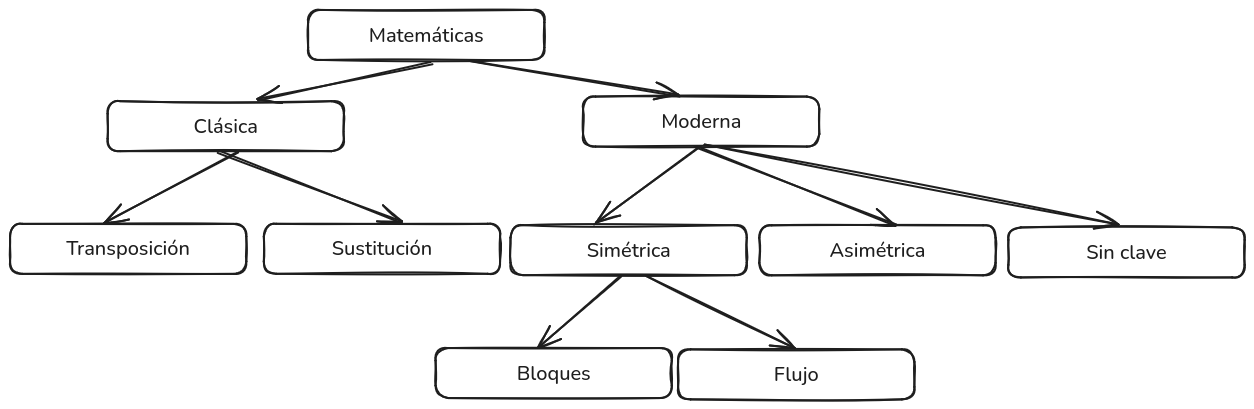
\includegraphics[width=0.8\textwidth]{imagenes/Clasificación_criptografía.png}
    \caption{Clasificación de la criptografía en función del método de cifrado}
    \label{fig:clasificacion_criptografia}
\end{figure}

\section{Estructura de un criptosistema}

Un criptosistema se define formalmente como la tupla
\[
  \bigl(\mathcal M,\;\mathcal C,\;\mathcal K,\;\mathcal E,\;\mathcal D\bigr),
\]
donde
\begin{itemize}
  \item \(\mathcal M\) es el espacio de texto plano.
  \item \(\mathcal C\) es el espacio de texto cifrado.
  \item \(\mathcal K\) es el espacio de claves.
  \item \(\mathcal E=\{E_k: k\in\mathcal K\}\) es el conjunto de funciones de cifrado \(E_k:\mathcal M\to\mathcal C\).
  \item \(\mathcal D=\{D_k: k\in\mathcal K\}\) es el conjunto de funciones de descifrado \(D_k:\mathcal C\to\mathcal M\).
\end{itemize}
Deben cumplirse las condiciones de corrección:
\[
  D_{k'}\bigl(E_k(M)\bigr)\;=\;M
  \quad\forall\,M\in\mathcal M,
\]
siendo \(k'\) la clave de descifrado asociada a la clave de cifrado \(k\).

\begin{figure}[H]
    \centering
    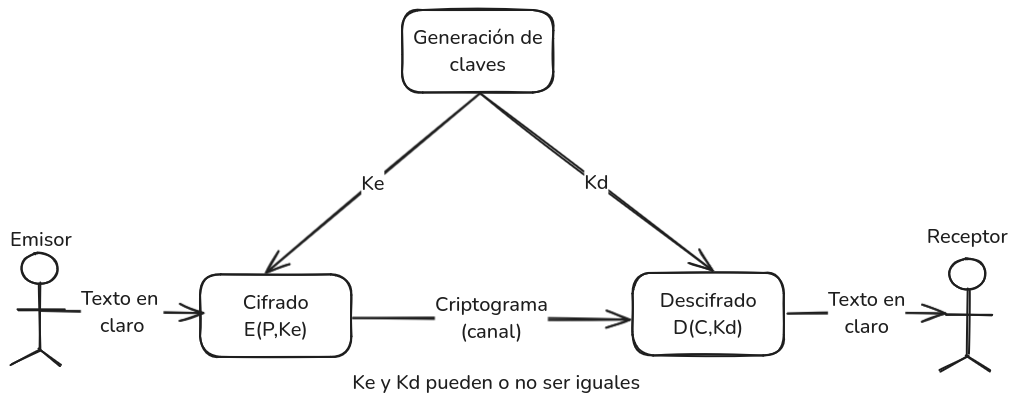
\includegraphics[width=0.8\textwidth]{imagenes/Esquema_criptosistema_cifrado_descifrado.png}
    \caption{Esquema de un criptosistema formal}
    \label{fig:esquema_criptosistema_cifrado_descifrado}
\end{figure}

\section{Criptografía sin clave o Funciones hash}
Las funciones hash son funciones unidireccionales de cálculo sencillo y eficiente, utilizadas para garantizar la integridad de los datos. Se aplican a un mensaje \(M\) produciendo un valor de longitud fija:
\[
  M \;\longmapsto\; H(M),
\]
donde \(H(M)\) suele tener 128, 160, 256 o 512 bits. Es computacionalmente inviable recuperar \(M\) a partir de \(H(M)\).

Una función hash criptográfica es una función eficiente que mapea cadenas binarias de longitud arbitraria a cadenas binarias de longitud fija \(n\). Para una función que produce valores de \(n\) bits, la probabilidad de que una cadena aleatoria termine en un valor dado es \(2^{-n}\). El valor de hash actúa como representante compacto de la cadena de entrada.

Para su uso en criptografía, \(H\) debe satisfacer al menos:

\begin{itemize}
  \item \textbf{Resistencia a preimagen:} Dado un valor \(y\) de \(n\) bits, resulta inviable encontrar \(x\) tal que \(H(x)=y\).
  \item \textbf{Resistencia a segunda preimagen:} Dado un mensaje \(x\), resulta inviable hallar otro \(x'\neq x\) con \(H(x')=H(x)\).
  \item \textbf{Resistencia a colisiones:} Resulta inviable encontrar dos entradas distintas \(x,y\) tales que \(H(x)=H(y)\).
\end{itemize}

Cuando \(H\) es público y sin clave, se le llama \emph{código de detección de modificaciones} (MDC). Si se añade una clave secreta al cómputo de hash, obtenemos un \emph{código de autenticación de mensaje} (MAC), que ofrece además autenticación del origen junto con integridad.

\subsection{MD5}
El MD5 (Message-Digest Algorithm 5) procesa el mensaje de entrada en bloques sucesivos de 512 bits y produce un resumen (digest) de 128 bits~\citep{IETF1321}.  
Su diseño sigue la construcción de Merkle–Damgard, inicializando cuatro registros de 32 bits y aplicando cuatro rondas de 16 operaciones cada una por bloque~\citep{Wang04_MD5}.  
En 2004 se demostró que MD5 ya no es resistente a colisiones: dos entradas diferentes pueden colisionar y producir el mismo digest en tiempo práctico~\citep{Wang04_MD5}.  
Por ejemplo, en 2009, Marc Stevens, Arjen Lenstra y Benne de Weger, un grupo de investigadores, construyeron colisiones con prefijos elegidos y generaron un certificado CA malicioso~\citep{Stevens09_MD5_CA}.  
Actualmente se desaconseja MD5 para cualquier uso criptográfico y se recomienda SHA-2 o SHA-3 como alternativas seguras~\citep{NIST_SP800131A}.


\subsection{SHA-1}
El SHA (Secure Hash Algorithm 1), fue publicado en 1995 como FIPS 180-1 por el NIST~\citep{FIPS1801}. Procesa los datos de entrada en bloques de 512 bits al igual que MD5, pero produce un digest de 160 bits con cinco registros de 32 bits y 80 rondas de mezcla~\citep{FIPS1801}. Su algoritmo es el siguiente:
\begin{enumerate}
    \item Se toma el mensaje original y se rellena hasta alcanzar una longitud de $448 \mod 512$ bits. Es decir, al dividir la longitud total entre 512, el resto debe ser 448.
    \item Se añade un campo de 64 bits que indica la longitud del mensaje original (incluyendo el propio relleno). Así, la longitud total del mensaje resultante, denotado $P'$, será un múltiplo de 512 bits.
    \item $P'$ se divide en bloques de longitud fija de 512 bits, denotados como $Y_1, Y_2, \ldots, Y_L$.
    \item Se inicia el cálculo del resumen. Cada bloque de 512 bits se mezcla con un búfer de 160 bits mediante 80 rondas. Cada 20 rondas se modifican las funciones de mezcla utilizadas. Este proceso continúa hasta procesar todos los bloques de entrada.
\end{enumerate}

Una vez terminado el cálculo, el buffer de 160 bits contiene el valor del compendio de mensaje. El SHA es $2^{32}$ veces más seguro que el MD5, pero su cálculo es más lento.

En 2005 Xiaoyun Wang y colaboradores redujeron la complejidad para hallar colisiones de \(2^{80}\) a \(2^{63}\) operaciones~\citep{Wang05_SHA1}, y en 2017 Google y CWI demostraron la primera colisión real de SHA-1 en el experimento \emph{SHAttered}~\citep{GoogleShattered}. El NIST anunció en 2011 la deprecación de SHA-1 y ha planificado retirarla completamente para fines de 2030~\citep{NIST_SP800131A}. Chrome dejó de aceptar certificados TLS firmados con SHA-1 en enero de 2017~\citep{ChromeDeprecateSHA1}, Mozilla Firefox siguió en febrero de 2017~\citep{MozillaDeprecateSHA1} y Microsoft finalizó el soporte para contenidos firmados con SHA-1 en 2021~\citep{MicrosoftSHA1Deprecation}.

\section{Criptografía de clave privada o simétrica}
Un cifrado simétrico utiliza una clave $k$ elegida de un espacio (conjunto) de claves posibles $K$ para cifrar un mensaje $m$ perteneciente al conjunto de mensajes posibles $M$, generando un texto cifrado $c \in C$.

El cifrado puede verse como una función:
\[
e : K \times m \rightarrow C
\]
cuyo dominio es el conjunto de pares $(k, m)$ y cuyo codominio es el espacio de textos cifrados $C$.

El descifrado se representa como una función:
\[
d : K \times C \rightarrow m
\]

Queremos que el descifrado revierta el cifrado:
\[
d(k, e(k, m)) = m \quad \forall k \in K, \forall m \in M
\]

Usando notación de subíndice para la clave, podemos escribir:
\[
e_k : m \rightarrow C \quad \text{y} \quad d_k : C \rightarrow m
\]
cumpliendo:
\[
d_k(e_k(m)) = m \quad \forall m \in M
\]

Esto implica que $e_k$ es una función inyectiva. Es decir, si $e_k(m) = e_k(m')$, entonces:
\[
m = d_k(e_k(m)) = d_k(e_k(m')) = m' \quad \forall k \in K, \forall m \in M
\]

\subsection*{Propiedades deseables de un cifrado simétrico}

Sea $(K, m, C, e, d)$ un sistema de cifrado. Este debe cumplir las siguientes propiedades:

\begin{enumerate}
    \item Para todo $k \in K$ y $m \in M$, debe ser fácil computar $e_k(m)$.
    \item Para todo $k \in K$ y $c \in C$, debe ser fácil computar $d_k(c)$.
    \item Dados uno o más textos cifrados $c_1, \ldots, c_n$ producidos con una misma clave $k$, debe ser computacionalmente difícil recuperar $d_k(c_1), \ldots, d_k(c_n)$ sin conocer $k$.
\end{enumerate}

Con este tipo de criptografía podemos garantizar la confidencialidad porque únicamente quien posea la llave secreta será capaz de ver el mensaje.
El problema con la criptografía simétrica es que si yo quisiera compartir secretos con n personas, para cada persona tendría que generar una nueva llave secreta.
Otro problema asociado con este tipo de criptografía es cómo comparto con otra persona de una forma confidencial e integra la llave secreta.
Estos problemas se resuelven de cierta manera con criptografía asimétrica.

\subsection{Cifrado de bloque}
Los cifrados de bloque cifran mensajes dividiéndolos en grupos de símbolos del mismo tamaño (bloques) y aplicando sobre cada uno de ellos un mismo algoritmo de cifra.

Llamamos \(B\) el tamaño de bloque del cifrado. Un mensaje de texto claro general consiste entonces en una lista de bloques de mensaje escogidos de \(M\), y la función de cifrado transforma estos bloques en una lista de bloques de texto cifrado en \(C\), donde cada bloque es una secuencia de \(B\) bits. Si el texto claro termina con un bloque de menos de \(B\) bits, rellenamos el final del bloque con ceros.

El cifrado y el descifrado se realizan bloque a bloque, por lo que basta estudiar el proceso para un único bloque de texto claro, es decir, para un solo \(m\in M\). Esto, por supuesto, explica la conveniencia de dividir un mensaje en bloques: un mensaje puede ser de longitud arbitraria, y resulta útil centrar el proceso criptográfico en una pieza de longitud fija. El bloque de texto claro \(m\) es una cadena de \(B\) bits, que para mayor concreción identificamos con el número correspondiente en forma binaria. En otras palabras, identificamos \(M\) con el conjunto de enteros \(m\) que satisfacen \(0 \le m < 2^B\) mediante
\[
\underbrace{m_{B-1}\,m_{B-2}\,\cdots\,m_2\,m_1\,m_0}_{\text{lista de \(B\) bits de \(m\)}}
\]

\[
\longleftrightarrow
\]

\[
\underbrace{m_{B-1}\cdot2^{B-1} + m_{B-2}\cdot2^{B-2} + \cdots + m_1\cdot2 + m_0}_{\text{entero entre 0 y \(2^B-1\)}}
\]

Aquí \(m_0,m_1,\dots,m_{B-1}\) son cada uno 0 o 1.

De manera similar, identificamos el espacio de claves \(K\) y el espacio de textos cifrados \(C\) con conjuntos de enteros correspondientes a cadenas de bits de un determinado tamaño de bloque. Para mayor simplicidad notacional, denotamos los tamaños de bloque para claves, textos claros y textos cifrados por \(B_k\), \(B_m\) y \(B_c\), respectivamente. No tienen por qué coincidir. Así, hemos identificado
\[
K = \{\,k \in \mathbb{Z} : 0 \le k < 2^{B_k}\}
\]

\[
M = \{\,m \in \mathbb{Z} : 0 \le m < 2^{B_m}\}
\]

\[
C = \{\,c \in \mathbb{Z} : 0 \le c < 2^{B_c}\}
\]


Surge de inmediato una pregunta importante: ¿qué tan grande debe ser el conjunto \(K\) que se debe de escoger, equivalentemente, qué tamaño de bloque de clave \(B_k\) se debería de elegir? Si \(B_k\) es demasiado pequeño, se puede probar cada número entre \(0\) y \(2^{B_k}-1\) hasta dar con la clave generada. Más precisamente, dado que se asume que se conoce el algoritmo de descifrado \(d\) (principio de Kerckhoffs), toma cada \(k\in K\) y calcula \(d_k(c)\). Suponiendo que se es capaz de distinguir entre textos claros válidos e inválidos, se acabará recuperando el mensaje.

Este ataque se conoce como ataque de búsqueda exhaustiva (o ataque de fuerza bruta), puesto que se explora exhaustivamente el espacio de claves. Con la tecnología actual, una búsqueda exhaustiva se considera inviable si el espacio tiene al menos \(2^{80}\) elementos. Por tanto, se debería de  escoger \(B_k \ge 80\).

Para muchos criptosistemas, existen refinamientos al ataque de búsqueda exhaustiva que sustituyen efectivamente el tamaño del espacio por su raíz cuadrada. Estos métodos se basan en el principio de que es más fácil encontrar objetos coincidentes (colisiones) en un conjunto que localizar un objeto en particular. Describimos algunos de estos ataques de "man-in-the-middle" o de colisiones en la sección 2.6. Si están disponibles ataques de este tipo, se deberá de escoger \(B_k \ge 160\).


Existen distintos modos de funcionamiento para los cifrados de bloques. El \emph{Electronic CodeBook} (ECB) y el \emph{Cipher-Block Chanining} (CBC) son dos de los modos más antiguos. Entre los sistemas de cifrado por bloques más conocidos están el Data Encryption Standard, Triple DES (3DES)\citep{tdes-techtarget}, Advanced Encryption Standard (AES)\citep{aes-nist} y Twofish\citep{Block_Cipher}\citep{twofish-schneier}.


\subsubsection{ECB}
El \emph{Electronic CodeBook} (ECB) es el modo de funcionamiento más sencillo del cifrado por bloques. Es más fácil porque se cifra directamente cada bloque de texto plano de entrada y la salida es en forma de bloques de texto cifrado. Generalmente, si un mensaje tiene un tamaño superior a $b$ bits, se puede dividir en un montón de bloques y repetir el procedimiento. En la figura se muestra un ejemplo de funcionamiento del mismo~\ref{fig:ECB_block_cypher}
\begin{figure}[H]
    \centering
    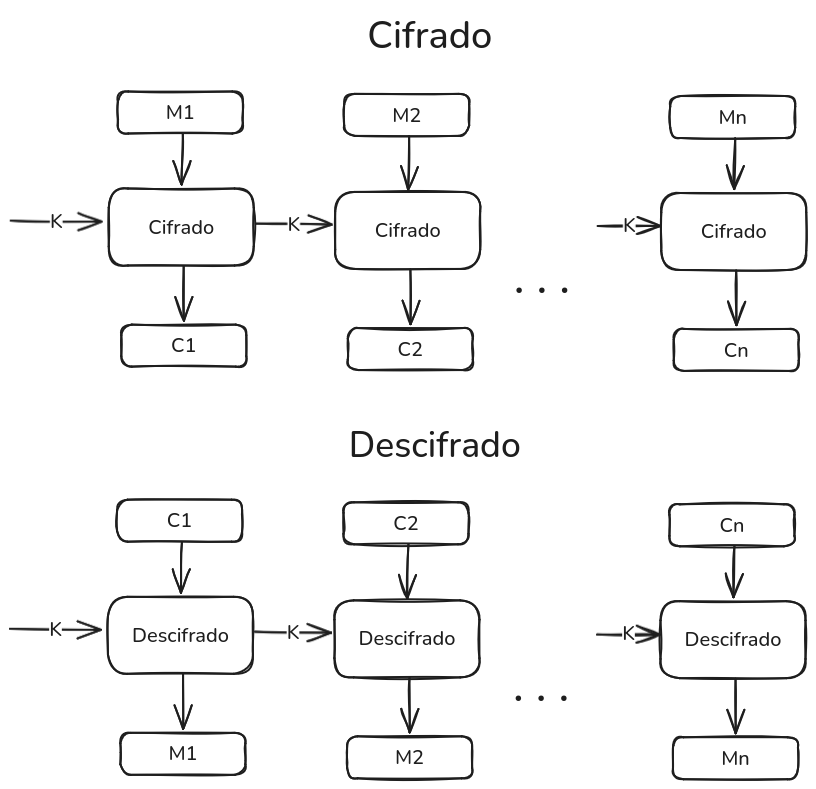
\includegraphics[width=0.8\textwidth]{imagenes/ECB_block_cypher.png}
    \caption{Ejemplo de cifrado y descifrado de bloque ECB}
    \label{fig:ECB_block_cypher}
\end{figure}

\subsubsection{CBC}
El modo \emph{Cipher Block Chaining} (CBC) mejora la seguridad del modo ECB al encadenar cada bloque cifrado con el siguiente. 
Antes de entrar en su explicación, en este modo se introduce un nuevo concepto:
Un IV es esencialmente otro input (además del texto plano $M$ y la llave $K$) usado para cifrar el texto. Es un bloque de datos, usado por varios modos de cifrado de bloques para introducir aleatoriedad en el proceso de cifrado para poder generar como resultado distintos textos cifrados incluso con el mismo texto plano cifrado varias veces.

No es necesario que sea secreto, pero si es necesario que no se vuelva a usar. Es recomendable que sea aleatorio, impredicible y de un único uso.
De forma simplificada:
\begin{itemize}
  \item Para cada bloque $M_i$ de texto claro:
    \[
      C_i = E\bigl(M_i \;\oplus\; C_{i-1},\,K\bigr)
    \]
    donde $C_{i-1}$ es el bloque cifrado anterior.
  \item Para el primer bloque, no existe $C_0$, por lo que se usa un vector de inicialización (IV) aleatorio:
    \[
      C_1 = E\bigl(M_1 \;\oplus\; \mathrm{IV},\,K\bigr).
    \]
  \item De este modo, incluso si $M_i = M_j$, normalmente $C_i \neq C_j$ porque $C_{i-1}\neq C_{j-1}$.
\end{itemize}

\subsection*{Pasos de cifrado}
\begin{enumerate}
  \item Calcular $X_1 = M_1 \oplus \mathrm{IV}$ y luego $C_1 = E(X_1, K)$.
  \item Para $i > 1$, calcular $X_i = M_i \oplus C_{i-1}$ y luego $C_i = E(X_i, K)$.
  \item Repetir hasta procesar todos los bloques de texto claro.
\end{enumerate}

\subsection*{Pasos de descifrado}
\begin{enumerate}
  \item Descifrar $D_1 = D(C_1, K)$ y obtener $M_1 = D_1 \oplus \mathrm{IV}$.
  \item Para $i > 1$, descifrar $D_i = D(C_i, K)$ y obtener $M_i = D_i \oplus C_{i-1}$.
  \item Repetir hasta recuperar todos los bloques de texto original.
\end{enumerate}

En la figura se muestra un ejemplo de funcionamiento del mismo~\ref{fig:CBC_block_cypher}
\begin{figure}[H]
    \centering
    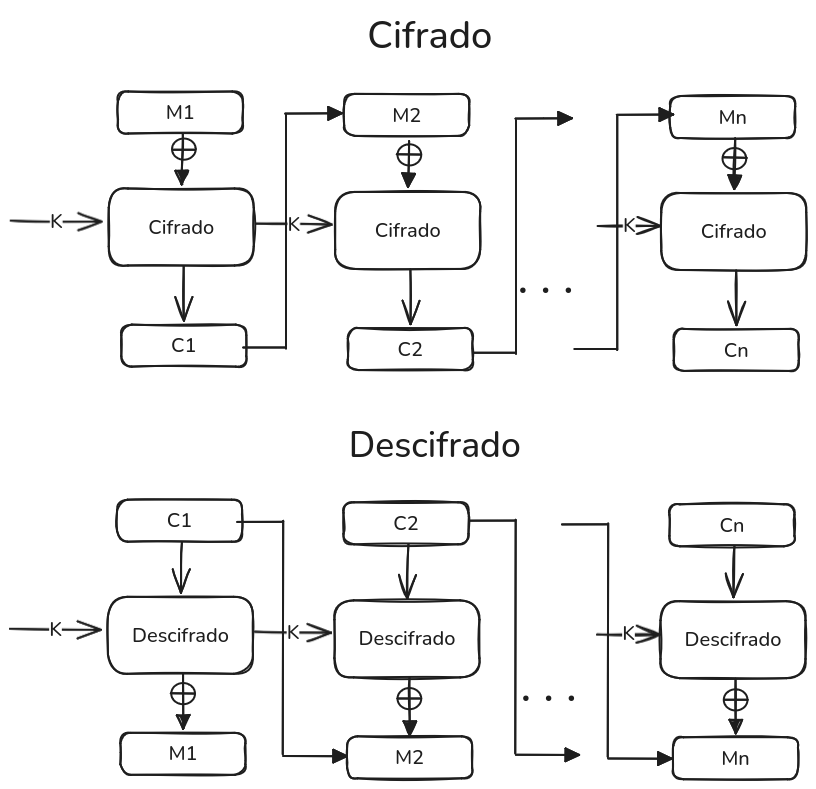
\includegraphics[width=0.8\textwidth]{imagenes/CBC_block_cypher.png}
    \caption{Ejemplo de cifrado y descifrado de bloque CBC}
    \label{fig:CBC_block_cypher}
\end{figure}

Una desventaja del mismo es que si se reutiliza el mismo IV para dos mensajes idénticos, se obtendrán los mismos bloques $C_1$, lo que compromete seguridad\cite{Block_Cipher}.

\subsection{Cifrado de flujo}
Los cifrados de flujo son ciertamente cifrados de bloque con una longitud de bloque igual a uno. Lo que los hace útiles es que la transformación de cifrado puede cambiar para cada símbolo del texto plano que se cifra.También pueden usarse cuando los datos deben procesarse símbolo por símbolo (por ejemplo, si el equipo no dispone de memoria o el almacenamiento intermedio es limitado).

Sea $K$ el espacio de claves. Una secuencia de símbolos $e_1e_2e_3\ldots \in K$ se denomina \textbf{flujo de claves} o \textit{keystream}.

Sea $A$ un alfabeto de $q$ símbolos, y sea $E_e$ un cifrado por sustitución simple con longitud de bloque 1, donde $e \in K$. Dado un texto claro $m_1m_2m_3\ldots$ y un flujo de claves $e_1e_2e_3\ldots$, un cifrado de flujo produce un texto cifrado $c_1c_2c_3\ldots$ tal que:

\[
c_i = E_{e_i}(m_i)
\]

Si $d_i$ denota la función inversa de $e_i$, entonces:

\[
D_{d_i}(c_i) = m_i
\]

Este tipo de criptografía se basa en hacer un cifrado bit a bit, esto se logra usando la operación XOR. Se utiliza un algoritmo determinístico que genera una secuencia pseudoaletoria de bits que junto con los bits del mensaje se van cifrando utilizando la operación XOR.

Un ejemplo de ello es el cifrado de vernam~\citep{vernam}, definido sobre $A = \{0, 1\}$. Dado un mensaje binario $m_1m_2\ldots m_t$ y una clave binaria $k_1k_2\ldots k_t$ de la misma longitud, el texto cifrado es:

\[
c_i = m_i \oplus k_i, \quad 1 \leq i \leq t
\]

Si la clave es aleatoria y no se reutiliza, se denomina \textbf{one-time pad}.

\textbf{Observación:} Hay dos cifrados por sustitución posibles sobre $A$:
\begin{itemize}
    \item $E_0$: $0 \mapsto 0$, $1 \mapsto 1$
    \item $E_1$: $0 \mapsto 1$, $1 \mapsto 0$
\end{itemize}

El flujo de claves determina cuál se aplica a cada símbolo.

Algunos ejemplos de cifrado de flujo son RC4 (usado en redes inalámbricas)\cite{rc4-ietf,rc4-gfg} y A5 (usado en
telefonía celular)\cite{a5-nop,a5-ucsb}.

\section{Criptografía de clave pública o asimétrica}
Si Alice y Bob quieren intercambiar mensajes usando un cifrado simétrico, deben primero acordar mutuamente una clave secreta \(k\). Esto es factible si tienen la oportunidad de reunirse en secreto o si pueden comunicarse una vez por un canal seguro. Pero ¿qué ocurre si no disponen de esa oportunidad y cada comunicación entre ellos es vigilada por su adversaria Eva? ¿Es posible que Alice y Bob intercambien una clave secreta en estas condiciones?

La primera reacción de la mayoría es que no es posible, ya que el intruso ve cada fragmento de información que intercambian. Fue la brillante intuición de Diffie y Hellman que, bajo ciertas hipótesis, sí lo es. La búsqueda de soluciones eficientes (y demostrables) a este problema, denominado criptografía de clave pública (o asimétrica), constituye una de las partes más interesantes de la criptografía matemática.

Definimos espacios de claves \(K\), de textos claros \(M\) y de textos cifrados \(C\). Sin embargo, un elemento \(k\) del espacio de claves es en realidad un par de claves,
\[
k = \bigl(k_{\text{priv}},\,k_{\text{pub}}\bigr),
\]
denominadas clave privada y clave pública, respectivamente. Para cada clave pública \(k_{\text{pub}}\) existe una función de cifrado correspondiente
\[
e_{k_{\text{pub}}}: M \longrightarrow C,
\]
y para cada clave privada \(k_{\text{priv}}\) existe una función de descifrado correspondiente
\[
d_{k_{\text{priv}}}: C \longrightarrow M.
\]
Estas funciones cumplen que si el par \(\bigl(k_{\text{priv}},\,k_{\text{pub}}\bigr)\) pertenece al espacio de claves \(K\), entonces
\[
d_{k_{\text{priv}}}\bigl(e_{k_{\text{pub}}}(m)\bigr) = m
\quad\forall\,m \in M.
\]

Para que un cifrado asimétrico sea seguro, debe resultar difícil para el intruso calcular la función de descifrado \(d_{k_{\text{priv}}}(c)\), incluso si conoce la clave pública \(k_{\text{pub}}\). Bajo esta suposición, Alice puede enviar \(k_{\text{pub}}\) a Bob mediante un canal inseguro, y Bob puede devolver el texto cifrado \(e_{k_{\text{pub}}}(m)\) sin temor a que el intruso lo descifre. Para poder descifrar, es necesario conocer la clave privada \(k_{\text{priv}}\), y, presumiblemente, solo Alice dispone de ella. A esta clave privada a veces se le llama información de \emph{trapdoor} de Alice, porque proporciona una vía directa para calcular la función inversa de \(e_{k_{\text{pub}}}\). El hecho de que las claves de cifrado y descifrado (\(k_{\text{pub}}\) y \(k_{\text{priv}}\)) sean diferentes confiere al cifrado su carácter asimétrico, de ahí su nombre.

Resulta fascinante que Diffie y Hellman concibieran este concepto sin contar con un par concreto de funciones; no obstante, sí propusieron un método análogo por el cual Alice y Bob pueden intercambiar de forma segura un dato aleatorio cuyo valor no conocen inicialmente. Describimos el método de intercambio de claves de Diffie y Hellman en la Sección ~\ref{sec:diffie_hellman} y, a continuación, analizaremos más adelante varios cifrados asimétricos como RSA (Sección~) y ECC (Sección~), cuya seguridad se fundamenta en la dificultad presunta de distintos problemas matemáticos.

\begin{figure}[H]
    \centering
    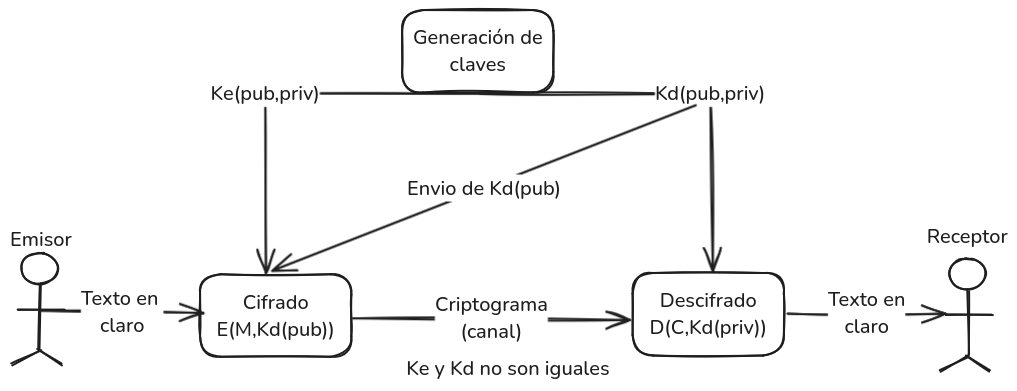
\includegraphics[width=0.8\textwidth]{imagenes/Cifrado_asimetrico.png}
    \caption{Ejemplo de cifrado asimétrico}
    \label{fig:cifrado_asimetrico}
\end{figure}

\subsection{Intercambio de claves Diffie–Hellman}\label{sec:diffie_hellman}
Como hemos mencionado anteriormente, el protocolo de Diffie-Hellman, publicado en 1976 \cite{diffie-hellman}, resuelve el problema de dos entidades que desean compartir una clave secreta para usar en un cifrado simétrico, pero su único canal de comunicación es inseguro y todo lo que intercambian lo observa el intruso. ¿Cómo pueden establecer una clave que el intruso no pueda deducir? La brillante idea de Diffie y Hellman fue aprovechar la dificultad del problema del logaritmo discreto en \(\mathbb{F}_p^*\). A continuación, se muestra el procedimiento del mismo:

\begin{enumerate}
  \item Alice y Bob acuerdan públicamente un primo grande \(p\) y un generador \(g\) de \(\mathbb{F}_p^*\).  
  \item Alice elige en secreto un entero \(a\) y calcula
    \[
      A \;\equiv\; g^a \pmod p.
    \]
  \item Bob elige en secreto un entero \(b\) y calcula
    \[
      B \;\equiv\; g^b \pmod p.
    \]
  \item Intercambian \(A\) y \(B\) por el canal público. Eve conoce \(p,g,A,B\).  
  \item Alice calcula la clave compartida
    \[
      K = B^a \equiv g^{ba} \pmod p,
    \]
    y Bob calcula
    \[
      K = A^b \equiv g^{ab} \pmod p.
    \]
\end{enumerate}

\begin{table}[H]
  \centering
  \begin{tabular}{p{4cm}p{8cm}}
    \toprule
    \textbf{Fase} & \textbf{Operación} \\
    \midrule
    Intercambio: elegir $p$ y $g$ & Un tercero de confianza elige y publica un primo \(p\) grande y un generador \(g\) de orden primo en \(\mathbb{F}_p^*\). \\
    Generación de claves secretas  & Alice elige \(a\), calcula \(A\equiv g^a\pmod p\); Bob elige \(b\), calcula \(B\equiv g^b\pmod p\). \\
    Intercambio público & Alice envía \(A\) a Bob, Bob envía \(B\) a Alice. \\
    Cálculos finales    & Alice calcula \(K\equiv B^a\pmod p\); Bob calcula \(K\equiv A^b\pmod p\). \\
    \bottomrule
  \end{tabular}
  \caption{Resumen del intercambio de claves Diffie–Hellman}
  \label{tab:dh-algoritmo}
\end{table}

\begin{ejemplo}
Supongamos que Alice y Bob acuerdan \(p=7\) y \(g=5\).  
Alice elige \(a=3\) y calcula
\[
  A = 5^3 \equiv 125 \equiv 6 \pmod 7,
\]
mientras que Bob elige \(b=4\) y obtiene
\[
  B = 5^4 \equiv 625 \equiv 2 \pmod 7.
\]
Tras intercambiar \(A=6\) y \(B=2\), ambos calculan
\[
  K = 2^3 \equiv 8 \equiv 1 \pmod 7,
  \quad
  K = 6^4 \equiv 1296 \equiv 1 \pmod 7,
\]
de modo que la clave compartida es \(K=1\).  
El intruso ve \(p,g,A,B\) pero, para calcular \(K=g^{ab}\), tendría que resolver el problema del logaritmo discreto en \(\mathbb{F}_7^*\), lo cual es prácticamente imposible cuando \(p\) tiene cientos de dígitos.
\end{ejemplo}

\subsection{Firma digital}
TODO: preguntar si es necesario esta seccion

\section{Resumen comparativo}
Los sistemas criptográficos actuales suelen combinar ambas: por ejemplo, se utiliza un esquema de clave pública para establecer una clave de sesión y luego un cifrado simétrico para procesar los datos.   

Hasta la fecha, la encriptación de clave pública es sustancialmente más lenta que la simétrica; sin embargo, no existe prueba de que deba serlo necesariamente. En la práctica, los puntos clave son:  
\begin{enumerate}
  \item La criptografía de clave pública facilita la firma eficiente, el no repudio) y la gestión de claves.  
  \item La criptografía de clave simétrica es muy eficiente para cifrar datos y para aplicaciones de integridad.  
\end{enumerate}

\paragraph{Observación (tamaños de clave)}  
Para lograr un nivel de seguridad equivalente, las claves privadas en sistemas de clave pública (por ejemplo, 2048 o 3072 bits en RSA) deben ser mucho más largas que las secretas en sistemas simétricos (por ejemplo, 128 bits en AES). Esto se debe a que, mientras que el ataque más eficiente contra la simétrica es la búsqueda exhaustiva, los sistemas de clave pública conocidos admiten algoritmos \emph{atajo} (por ejemplo, factorización) más eficientes que el barrido completo del espacio de claves. Por tanto, para igualar los 128 bits simétricos, se requieren claves RSA de unos 3072 bits, es decir, más de 24 veces más largas, aunque valores del orden de 10 veces mayores se citan frecuentemente en la literatura~\citep{SecurityStrengthRSA}.

\section{Principios de diseño criptográfico}

En 1883, Auguste Kerckhoffs~\cite{Petitcolas2011Kerckhoffs} formuló seis principios esenciales para el diseño de sistemas criptográficos:

\begin{enumerate}
  \item Debe ser, cuanto menos, imposible de romper en la práctica.
  \item La seguridad no debe depender del secreto del algoritmo, sino únicamente de la clave.
  \item La clave debe poder ser almacenada, pudiendo ser reemplazable.
  \item El texto cifrado debe poder transmitirse sin errores por medios estándar.
  \item El sistema debe ser portátil y operable por una sola persona.
  \item El sistema debe ser fácil de usar, sin requerir un esfuerzo mental excesivo.
\end{enumerate}
\section{Seguridad y modelos de ataque}

La seguridad de un sistema criptográfico se evalúa frente a distintos modelos de ataque, que describen el acceso y las capacidades del adversario. A grandes rasgos, estos modelos se agrupan en:

\subsection{Ataques pasivos y activos}

\begin{description}
  \item[Ataques pasivos:] El atacante únicamente observa el tráfico cifrado (o el sistema) sin modificarlo. Incluyen la intercepción de mensajes y el análisis de tráfico, en los que se extrae información de patrones de comunicación \cite{different_types_cryptography_attacks}\cite{active_and_passive_attacks_in_information_security}.
  \item[Ataques activos:] El atacante altera, inyecta o interfiere el flujo de datos. Ejemplos típicos son el man-in-the-middle (interposición entre emisor y receptor) y la modificación de mensajes en tránsito \cite{what_are_cryptographic_attacks}.
\end{description}

\subsection{Modelos clásicos de criptoanálisis}

\begin{itemize}
  \item \emph{Ataque por texto cifrado únicamente (COA):} El atacante dispone solo del texto cifrado. Es el escenario más realista pero también el más limitado.
  \item \emph{Fuerza bruta (exhaustiva):} Se calculan y prueban todas las claves posibles hasta dar con la correcta. Su dificultad depende únicamente del tamaño de la clave \cite{cryptography_attacks_6_types_and_prevention}\cite{types_of_cryptographic_attacks_to_know}.
  \item \emph{Ataque con texto plano conocido (KPA):} Se accede a uno o varios pares (texto plano, texto cifrado), lo que permite reducir el espacio de búsqueda.
  \item \emph{Ataque por texto plano elegido (CPA):} El atacante elige ciertos textos para cifrar y obtiene sus correspondientes cifrados. Es fundamental en la seguridad de sistemas de clave pública.
  \item \emph{Ataque adaptativo por texto plano elegido (CPA2):} Variante de CPA donde el atacante decide nuevos textos a cifrar tras ver resultados anteriores.
  \item \emph{Ataque por texto cifrado elegido (CCA):} El atacante puede descifrar libremente ciertos cifrados de su elección, obteniendo los planos resultantes.
  \item \emph{Ataque adaptativo por texto cifrado elegido (CCA2):} Versión más poderosa de CCA, donde cada descifrado elegido se basa en análisis previos.
\end{itemize}

\subsection{Ataques avanzados}

\begin{itemize}
  \item \emph{Canal lateral (side-channel):} Se explota información derivada de la implementación (tiempos, consumo eléctrico, emisiones electromagnéticas) para inferir claves \cite{cryptanalysis_and_types_of_attacks}.
  \item \emph{Ataque de clave relacionada (related-key):} El atacante conoce cifrados de textos planos bajo claves que guardan alguna relación matemática con la clave objetivo.
  \item \emph{Sesgo estadístico (bias attacks):} Se buscan patrones no aleatorios en la generación de claves o estados intermedios para acotar posibles valores \cite{modern_cryptographic_attacks_guide_for_perplexed}.
  \item Ataque \emph{Evil Maid}: Consiste en acceso físico al dispositivo para instalar malware o keyloggers y robar claves cuando el usuario no está presente.
\end{itemize}
%\chapter{Introducción a la Computación Cuántica}

\section{Fundamentos de la mecánica cuántica}
\subsection{El qubit: superposición y coherencia}
\subsection{Entrelazamiento cuántico}

\section{Circuitos Cuánticos}
\subsection{Puertas cuánticas}
\subsubsection{Puertas de un solo qubit (Hadamard)}
\subsubsection{Puertas de múltiples qubits (CNOT)}
\subsection{Medición de un Qubit}

\section{Algoritmos cuánticos clásicos}
\subsection{Algoritmo de Grover para búsqueda}
\subsection{Algoritmo de Shor para factorización}
\chapter{Campos finitos}
La aritmética en campos finitos es fundamental para numerosos algoritmos de clave pública, incluidos los basados en el problema del logaritmo discreto en campos finitos, los esquemas de curvas elípticas y las aplicaciones emergentes de curvas hiperelípticas. El rendimiento de estos protocolos depende en gran medida de nuestra capacidad para realizar rápidamente operaciones básicas en el campo subyacente.  

Los campos finitos (también llamados cuerpo finito o cuerpo de Galois) se denotan como \(\mathrm{GF}(p^m)\), donde \(p\) es un número primo y \(m\) un entero positivo. Para que los sistemas de curvas elípticas sean eficientes, es imprescindible implementar de manera óptima la suma, la resta, la multiplicación y la inversión en dicho campo. Existen tres familias de campos que resultan especialmente adecuadas para ECC (Criptografía de Curvas Elípticas):  
\begin{itemize}
  \item \textbf{Campos primos} (\(\mathbb{F}_p\)),  
  \item \textbf{Campos binarios} (\(\mathbb{F}_{2^m}\)),  
  \item \textbf{Campos de extensión óptima} (OEF).  
\end{itemize}
En las secciones siguientes se presenta una introducción informal a la teoría de campos finitos y se describen en detalle los algoritmos eficientes para cada tipo de campo.  

Dado que en muchas aplicaciones los tamaños de \(p^m\) son muy grandes, entender la complejidad computacional de estas operaciones es clave para evaluar el rendimiento global de los esquemas criptográficos basados en curvas elípticas.  

Nota: $GF(p^m)$ == \(\mathbb{F}_{p^m}\).

\section{Introducción a campos finitos}
Los campos son abstracciones de sistemas numéricos familiares (como los racionales \(\mathbb{Q}\), los reales \(\mathbb{R}\) o los complejos \(\mathbb{C}\)) que reúnen ciertas propiedades esenciales. Un campo \(\mathbb{F}\) consta de un conjunto \(\mathbb{F}\) junto con dos operaciones, suma (\(+\)) y producto (\(\cdot\)), que satisfacen:

\begin{enumerate}
  \item $(\mathbb{F},+)$ es un grupo abeliano con identidad suma denotada por $0$.
  \item $(\mathbb{F}\setminus\{0\},\cdot)$ es un grupo abeliano con identidad multiplicativa denotada por $1$.
  \item La multiplicación distribuye sobre la suma:
    \[
      (a + b)\cdot c = a\cdot c + b\cdot c
      \quad\text{para todo }a,b,c\in\mathbb{F}.
    \]
\end{enumerate}

Si el conjunto \(\mathbb{F}\) es finito, se dice que el campo es finito.  

En un campo, la resta se define mediante la suma de inversos aditivos: para \(a,b\in\mathbb{F}\),  
\[
  a - b \;=\; a + (-b),
\]
donde \(-b\) es el elemento único que satisface \(b + (-b) = 0\).  

La división se define usando el inverso multiplicativo: para \(a,b\in\mathbb{F}\) con \(b\neq0\),
\[
  \frac{a}{b} \;=\; a \cdot b^{-1},
\]
siendo \(b^{-1}\) el único elemento que cumple \(b\cdot b^{-1}=1\).  

El \emph{orden} de un campo finito es el número de sus elementos. Existe un campo finito de orden \(q\) si y solo si \(q\) es una potencia prima, es decir, \(q = p^m\) con \(p\) primo (característica del campo) y \(m\) entero positivo.  

\begin{itemize}
  \item Si \(m=1\), el campo se llama \emph{campo primo} y se denota \(\mathbb{F}_p\).  
  \item Si \(m\ge2\), se llama \emph{campo de extensión} y se denota \(\mathbb{F}_{p^m}\).  
\end{itemize}

Para cada potencia prima \(q\), existe esencialmente un único campo finito de orden \(q\): todos ellos son isomorfos (idénticos en estructura, aunque difiera la representación de sus elementos). Por ello se usa la notación general \(\mathbb{F}_q\).  



\section{Aritmética en \texorpdfstring{$\mathbb{F}_p$}{Fp}}
Sea $p$ un número primo. El conjunto
$$
  \mathbb{F}_p = \{0,1,2,\dots,p-1\},
$$
con las operaciones de suma y multiplicación módulo $p$, $\mathbb{Z}/p\mathbb{Z}$, constituye un campo finito de orden $p$. Denotaremos este campo por $\mathbb{F}_p$ y llamaremos a $p$ el \emph{módulo} de $\mathbb{F}_p$. Para cualquier entero $a$, $a \bmod p$ denota el único residuo $r$, $0\le r\le p-1$, obtenido al dividir $a$ por $p$; esta operación se llama \emph{reducción módulo $p$}.

Todos los elementos no nulos de $\mathbb{F}_p$ tienen inverso multiplicativo, y forman un grupo cíclico de orden $p-1$ (esto es una consecuencia del pequeño Teorema de Fermat).

\paragraph{Ejemplo 2.1 (campo primo $\mathbb{F}_{31}$)}  
Los elementos de $\mathbb{F}_{31}$ son $\{0,1,2,\dots,30\}$. A continuación se muestran algunas operaciones en $\mathbb{F}_{31}$:

\begin{enumerate}
  \item \textbf{Suma:} $9 + 25 = 34 \equiv 3 \pmod{31}.$
  \item \textbf{Resta:} $9 - 25 = -16 \equiv 15 \pmod{31}.$
  \item \textbf{Multiplicación:} $9 \cdot 25 = 225 \equiv 8 \pmod{31}.$
  \item \textbf{Inverso multiplicativo:} $9^{-1} = 7$ ya que $9 \cdot 7 = 63 \equiv 1 \pmod{31}.$
\end{enumerate}

\section{Aritmética en \texorpdfstring{$\mathbb{F}_{2^m}$}{F2m}}
Los campos finitos de orden $2^m$, también llamados \emph{campos binarios}, se construyen como extensiones de polinomios:
\[
  \mathbb{F}_{2^m}\cong\mathbb{F}_2[x]/(f(x)),
\]
donde $f(x)$ es un polinomio irreducible de grado $m$ sobre $\mathbb{F}_2$.
En tal campo, cada elemento puede representarse como un polinomio de grado < $m$ con coeficientes en ${0,1}$ (equivalentemente, como un vector binario de $m$ bits).

\subsection{Representación polinomial}
Cada elemento se escribe como
\[
  a(x)=a_{m-1}x^{m-1}+\cdots+a_1x+a_0,\quad a_i\in\{0,1\}.
\]
La suma de elementos se realiza como la suma de polinomios coeficiente a coeficiente (operación equivalente a XOR bit a bit, sin acarreo), y la multiplicación se reduce módulo $f(x)$:
\[
  a(x)\cdot b(x)\bmod f(x).
\]
La reducción $p(x)\bmod f(x)$ es el residuo de grado < $m$ tras la división larga.

\paragraph{Ejemplo 2.2 (campo $\mathbb{F}_{2^3}$)}
Sea $f(x)=x^3+x+1$. Entonces
\[
  \mathbb{F}_{2^3}=\{0,1,x,x+1,x^2,x^2+1,x^2+x,x^2+x+1\}.
\]
\begin{enumerate}
  \item Suma: $(x^2+x+1)+(x+1)=x^2$.
  \item Multiplicación: $(x^2+x+1)(x+1)=x^3+x+1\equiv x+1\pmod{f(x)}$.
  \item Inverso: $(x^2+x+1)^{-1}=x^2$, pues $(x^2+x+1)x^2=x^4+x^3+x^2\equiv1\pmod{f(x)}$.
\end{enumerate}

\paragraph{Ejemplo 2.3 (isomorfismo de campos)}
Para $m=3$ hay dos irreducibles: $f_1(x)=x^3+x+1$ y $f_2(x)=x^3+x^2+1$. Los campos $\mathbb{F}_2[x]/(f_1)$ y $\mathbb{F}_2[x]/(f_2)$ tienen idénticos elementos y son isomorfos, pues existe un mapeo que envía la clase de $x$ en uno a una raíz de $f_1$ en el otro.

\section{Campos de extensión}
La representación por base polinomial para campos binarios se generaliza a todos los campos de extensión de la siguiente manera. Sea $p$ un primo y $m\ge2$. Denotamos por $\mathbb{F}_p[z]$ el anillo de polinomios en la variable $z$ con coeficientes en $\mathbb{F}_p$. Sea $f(z)\in\mathbb{F}_p[z]$ un polinomio irreducible de grado $m$—existen para cualquier par $(p,m)$ y pueden hallarse eficientemente (ver Apéndice A). La irreducibilidad significa que $f(z)$ no se factoriza como producto de polinomios en $\mathbb{F}_p[z]$ de grado menor que $m$. Entonces:
\[
  \mathbb{F}_{p^m}=\{a_{m-1}z^{m-1}+\cdots+a_1z+a_0:\,a_i\in\mathbb{F}_p\}
\]
con suma habitual de polinomios y producto reducido módulo $f(z)$.

\paragraph{Ejemplo 2.4 (campo $\mathbb{F}_{251^5}$)}
Sea $p=251$, $m=5$ y $f(z)=z^5+z^4+12z^3+9z^2+7$, irreducible en $\mathbb{F}_{251}[z]$. Entonces $\mathbb{F}_{251^5}$ consta de polinomios de grado \(<5\) con coeficientes en $\{0,1,\dots,250\}$. Por ejemplo, sean:
\[
  a=123z^4+76z^2+7z+4,\quad b=196z^4+12z^3+225z^2+76.
\]
\begin{enumerate}
  \item Suma: $a+b=68z^4+12z^3+50z^2+7z+80.$
  \item Resta: $a-b=178z^4+239z^3+102z^2+7z+179.$
  \item Multiplicación: $a\cdot b=117z^4+151z^3+117z^2+182z+217.$
  \item Inverso: $a^{-1}=109z^4+111z^3+250z^2+98z+85,$
\end{enumerate}
obeylines

\section{Grupos multiplicativos y orden de un elemento}
En todo campo finito $\mathbb{F}_q$, el conjunto $\mathbb{F}_q^*=\mathbb{F}_q\setminus\{0\}$ es un grupo cíclico de orden $q-1$. Un generador $g$ (elemento primitivo) cumple:
\[
  \langle g\rangle=\mathbb{F}_q^*,\quad g^k\neq1\text{ para }0<k<q-1.
\]
El \emph{orden} de $a\in\mathbb{F}_q^*$ es el menor $d>0$ tal que $a^d=1$. Determinarlo es clave al definir curvas elípticas seguras.



\part{Marco Teórico}
\chapter{Teoría de las curvas elípticas}

\section{Introducción y motivación}
Los investigadores llevaban años buscando funciones más seguras para criptografía y en 1985 se propuso por primera vez el uso de curvas elípticas como base del problema del logaritmo discreto en un grupo~\cite{Koblitz1987,Miller1986}. Se cree que las curvas elípticas ofrecen un nivel de seguridad equivalente al de RSA pero con tamaños de clave mucho menores. Para ilustrar la diferencia en términos intuitivos, comparemos la energía necesaria para romper los diferentes sistemas con la cantidad de agua que esa energía podría hervir~\cite{Rickard2016,Lenstra2000}:
\begin{itemize}
  \item Romper una clave RSA de 228 bits requiere menos energía que la necesaria para hervir una cucharadita de agua.  
  \item Romper una clave ECC de 228 bits equivaldría a la energía necesaria para hervir toda el agua de la Tierra.  
  \item Para obtener el mismo nivel de seguridad con RSA haría falta una clave de unos 2 380 bits, lo cual es muy ineficiente en entornos con recursos limitados.  
\end{itemize}

Como hemos mencionado anteriormente en el capítulo~\ref{chap:Campos_finitos}, la eficiencia de los esquemas basados en curvas elípticas depende directamente de la velocidad de los algoritmos de aritmética de curva, que a su vez recaen en las operaciones sobre el campo (suma, multiplicación, inversión)...

La figura~\ref{fig:ECDSA_esquema} muestra las bases necesarias para entender e implementar un protocolo como el algoritmo de firma digital de curva elíptica (ECDSA). La aritmética de curvas no solo se construye sobre las operaciones en el campo subyacente, sino que en algunos casos también requiere aritmética de grandes enteros y operaciones modulares. ECDSA emplea una función hash y ciertas operaciones modulares, pero los pasos más costosos desde el punto de vista computacional son las propias operaciones en la curva.
\begin{figure}[H]
    \centering
    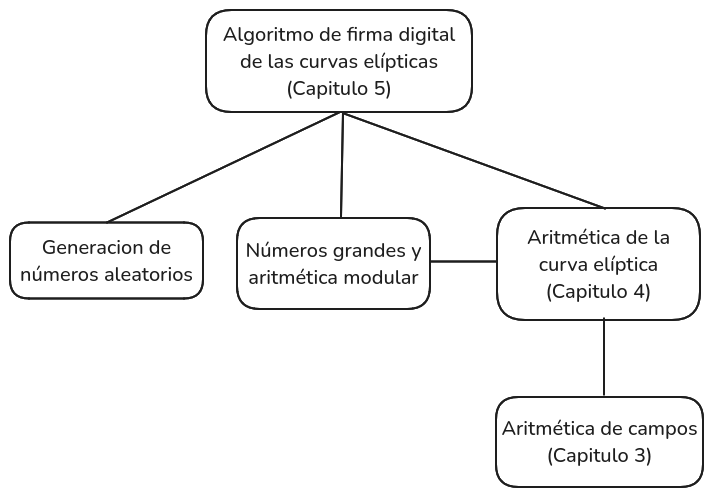
\includegraphics[width=0.8\textwidth]{imagenes/ECDSA_esquema.png}
    \caption{Esquema del Algoritmo de firma digital de las curvas elípticas (ECDSA)}
    \label{fig:ECDSA_esquema}
\end{figure}
%need to update this
La sección~\ref{sec:historia_curvas_elipticas} ofrece una introducción a las curvas elípticas donde se presentan las operaciones de grupo de suma y duplicado para los puntos de la curva, junto con su estructura fundamental y otras propiedades básicas. La sección~3.2 expone las representaciones en coordenadas proyectivas (y los algoritmos asociados de suma y duplicado), de especial interés cuando la inversión en el campo es más cara que la multiplicación. La sección~3.3 discute estrategias para la multiplicación de puntos.

Los métodos de las secciones~3.4, 3.5 y 3.6 están relacionados en que todos ellos explotan endomorfismos de la curva para reducir el coste del duplicado en la multiplicación de puntos. La sección~3.4 trata las curvas de Koblitz especiales, que permiten sustituir el duplicado de punto sobre \(\mathbb{F}_2\) por operaciones de cuadrado en el campo, mucho más baratas. La sección~3.5 examina una clase más amplia de curvas elípticas que admiten endomorfismos usados eficientemente para disminuir el número de duplicaciones. Las estrategias de la sección~3.6, para curvas sobre campos binarios, reemplazan la mayoría de los duplicados por una operación de “halving” de punto, potencialmente más rápida. La sección~3.7 recoge comparaciones de conteo de operaciones para métodos seleccionados de multiplicación de puntos. Finalmente, la sección~3.8 concluye con notas del capítulo y referencias.


\subsection{Historia y aplicaciones}\label{sec:historia_curvas_elipticas}
En 1997 Certicom lanzó el \emph{ECC Challenge} para evaluar la dificultad práctica del problema del logaritmo discreto en curvas elípticas~\cite{gaudry2007breaking}. Pocos años después, en 1998, el comité ANSI X9 publicó la norma X9.62 definiendo el algoritmo de firma ECDSA, marcando el primer estándar formal para firmas basadas en curvas elípticas~\cite{ansi_x962_1998}. 
En el año 2000, el NIST incorporó curvas elípticas en el FIPS 186–2 (Digital Signature Standard), consolidando su uso en aplicaciones gubernamentales y financieras~\cite{nist_fips186_2}.

En 2005 la NSA anunció la Suite B de algoritmos criptográficos, recomendando las curvas P-256, P-384 y P-521 para uso en comunicaciones seguras de nivel gubernamental~\cite{rfc5430}. Con la adopción de TLS 1.2 y la publicación del RFC 8422 en 2018, las curvas secp256r1 (también conocida como prime256v1) y X25519 se convirtieron en cimientos de la seguridad de Internet, al ofrecer un excelente equilibrio entre rendimiento y seguridad~\cite{rfc8422}.

Los esquemas de intercambio de clave ECDH y de firma ECDSA aprovechan la elevada seguridad por bit de las curvas, permitiendo, por ejemplo, igualar la fuerza de una clave RSA de 3072 bits con una curva de solo 256 bits~\cite{hankerson2004guide}.
Protocolos tan extendidos como TLS o SSH incluyen implementaciones de ECC, acelerando el establecimiento de sesiones seguras~\cite{rfc4492,rfc5656}. En sistemas distribuidos, Bitcoin emplea la curva secp256k1 para generar direcciones y validar transacciones, gracias a su rapidez y su seguridad criptográfica~\cite{wuille2017secp256k1}.

En entornos con recursos limitados, como dispositivos IoT o tarjetas inteligentes, ECC ha demostrado reducir consumo energético y acelerar operaciones criptográficas frente a RSA, al requerir menos ciclos de CPU y menos memoria~\cite{hodges2001implementing}. Además, las propiedades algebraicas de las curvas han sido la base para esquemas avanzados como sistemas de emparejamientos (pairing-based cryptography), identidades basadas en curva (IBE) y firmas Schnorr y EdDSA, ampliando enormemente el catálogo de construcciones criptográficas eficientes~\cite{boneh2001identity}.

\section{Definición de una curva elíptica}\label{sec:definicion_curvas_elipticas}

\subsection{Forma de Weierstrass general}\label{sec:weierstrass_curvas_elipticas}
\subsection{Transformaciones y cambios de coordenadas}

\section{Estructura de grupo}
\subsection{Punto en el infinito}
\subsection{Ley de suma de puntos (geometría proyectiva)}
\subsection{Propiedades algebraicas}

\section{Curvas sobre cuerpos finitos}\label{sec:curvas_sobre_cuerpos_finitos}
\subsection{Curvas sobre \texorpdfstring{$\mathbb{F}_p$}{Fp}}\label{sec:curvas_sobre_cuerpos_finitos_primos}
\subsection{Curvas binarias sobre \texorpdfstring{$\mathbb{F}_{2^m}$}{F2m}}\label{sec:curvas_sobre_cuerpos_finitos_binarios}

\section{Coordenadas y representación}\label{sec:coordenadas_curvas_elipticas}
\subsection{Coordenadas afines}
\subsection{Coordenadas proyectivas y Jacobianas}
\subsection{Coordenadas 'mixed' y optimizaciones}

\section{Selección de parámetros}
\subsection{Tamaños de curva y seguridad}
\subsection{Cofactores y subgrupos}
\subsection{Curvas estandarizadas (secp256k1, Curve25519, …)}
\chapter{Criptografía con curvas elípticas (ECC)}

\section{Fundamentos de ECC}
\subsection{Ventajas frente a RSA y DH}
\subsection{Comparativa de tamaños de clave}

\section{Intercambio de claves: ECDH}
\subsection{Protocolo básico}
\subsection{Variantes y extensiones (X25519, etc.)}

\section{Firmas digitales: ECDSA}
\subsection{Generación y verificación de firma}
\subsection{Problemas prácticos (k reutilizado, mal RNG)}

\section{Otras construcciones criptográficas}
\subsection{ECIES: cifrado híbrido}
\subsection{EdDSA: firmas deterministas sobre edwards}

\section{Aspectos de implementación}
\subsection{Resistencia a canal lateral}
\subsection{Bibliotecas y hardware acelerado}

\section{Estándares y recomendaciones}
\subsection{NIST, SECG, RFCs relevantes}
\subsection{Buenas prácticas de despliegue}
\part{Implementación y Experimentación}
%\input{capitulos/06_Implementacion}
%\input{capitulos/07_Pruebas}

\part{Conclusión}
%\input{capitulos/08_Conclusiones}
%
%%\chapter{Conclusiones y Trabajos Futuros}
%
%
%%\nocite{*}
%\bibliography{bibliografia/bibliografia}\addcontentsline{toc}{chapter}{Bibliografía}
%\bibliographystyle{miunsrturl}
%
% ----------------------------------------------------------------------------------
% Bibliografía
% ----------------------------------------------------------------------------------
\cleardoublepage
\phantomsection
\addcontentsline{toc}{chapter}{Bibliografía}
\bibliographystyle{plainnat}
\bibliography{bibliografia/bibliografia}
\section*{Otro material}
\begin{itemize}
  \item Diversas consultas puntuales al sitio \emph{StackOverFlow}.
  \item Material docente de las asignaturas Álgebra Lineal y Estructuras Matemáticas, Metodología de la Programación, Aprendizaje Automático y Fundamentos de Redes impartidas en el Grado de Ingeniería Informática en la Universidad de Granada.
\end{itemize}

% Añadir marcador manual a la entrada deseada
\phantomsection
\label{vernam-ref}


\appendix
%\input{apendices/manual_usuario/manual_usuario}
%%\input{apendices/paper/paper}
%\input{glosario/entradas_glosario}
% \addcontentsline{toc}{chapter}{Glosario}
% \printglossary
\chapter*{}
\thispagestyle{empty}

\end{document}
